% -*- mode: latex; mode: flyspell; ispell-local-dictionary: "en_US"; coding: utf-8 -*-

\documentclass{standalone}

\usepackage[utf8]{inputenc}
\usepackage[english]{babel}

\usepackage{amsmath,amsfonts,amssymb}

\usepackage{tikz,pgfplots}
\usetikzlibrary{plotmarks}
\pgfplotsset{compat=newest}

\usepgfplotslibrary{groupplots}
\pgfplotsset{every axis/.style={scale only axis}}

\pgfplotsset{
  major grid style={dashed},
  minor grid style={thin,dotted},
  ymajorgrids,
  yminorgrids,
  every axis/.append style={
    line width=0.7pt,
    tick style={
      line cap=round,
      thin,
      major tick length=4pt,
      minor tick length=2pt,
    },
  },
  legend cell align=left,
  legend style={
    line width=0.7pt,
    /tikz/every even column/.append style={column sep=3mm,black},
    /tikz/every odd column/.append style={black},
  },
  % move title closer
  legend style={font=\small},
  title style={yshift=-2pt},
  % less space on left and right
  enlarge x limits=0.04,
  every tick label/.append style={font=\footnotesize},
  every axis label/.append style={font=\small},
  every axis y label/.append style={yshift=-1ex},
  /pgf/number format/1000 sep={},
  axis lines*=left,
  xlabel near ticks,
  ylabel near ticks,
  axis lines*=left,
  label style={font=\footnotesize},       
  tick label style={font=\footnotesize},
  plotConstructionWoRs/.style={
    width=38mm,
    height=38mm,
    only marks,
    ymin=9,
    ymax=2000,
  },
}


\usepackage{xcolor}
\definecolor{my-dark-red}{RGB}{183, 28, 28}
\definecolor{my-red}{RGB}{244,67,54}
\definecolor{my-pink}{RGB}{233,30,99}
\definecolor{my-purple}{RGB}{156,39,176}
\definecolor{my-deep-purple}{RGB}{103,58,183}
\definecolor{my-indigo}{RGB}{63,81,181}
\definecolor{my-blue}{RGB}{33,150,243}
\definecolor{my-light-blue}{RGB}{3,169,244}
\definecolor{my-cyan}{RGB}{0,188,212}
\definecolor{my-teal}{RGB}{0,150,136}
\definecolor{my-green}{RGB}{76,175,80}
\definecolor{my-light-green}{RGB}{139,195,74}
\definecolor{my-lime}{RGB}{205,220,57}
\definecolor{my-yellow}{RGB}{255,235,59}
\definecolor{my-amber}{RGB}{255,193,7}
\definecolor{my-orange}{RGB}{255,152,0}
\definecolor{my-deep-orange}{RGB}{255,87,34}
\definecolor{my-brown}{RGB}{121,85,72}
\definecolor{my-grey}{RGB}{158,158,158}
\definecolor{my-blue-grey}{RGB}{96,125,139}
\definecolor{my-lipics-grey}{rgb}{0.6,0.6,0.61}


\colorlet{fp1Color}{my-blue}
\colorlet{fpzColor}{my-blue}
\colorlet{lpf1Color}{my-green}
\colorlet{lpfzColor}{my-green}
\colorlet{lpf1dpColor}{my-deep-orange}
\colorlet{lpfzdpColor}{my-deep-orange}
\colorlet{belazzouguiColor}{my-dark-red}

\begin{document}

% IMPORT-DATA our_stats ./data/repetitive_our.txt
% IMPORT-DATA belazzougui_stats ./data/repetitive_belazzougui.txt
% IMPORT-DATA algorithm_meta_data ./data/algorithm_names.txt

%% SQL DELETE FROM our_stats WHERE algorithm LIKE 'FP-pruning-z'

\begin{tabular}{lll}
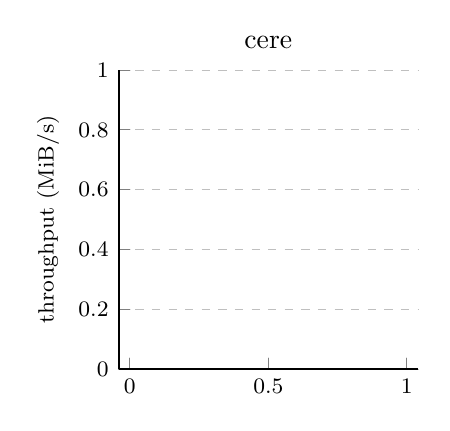
\begin{tikzpicture}
\begin{axis}[
  title={cere},
  ylabel={throughput (MiB/s)},
  %ymode=log,
  plotConstructionWoRs,
  legend to name={leg:construction_with_rs}
]
%% MULTIPLOT(algorithm|attr|ptitle)
%% SELECT (space_usage*8.0)/prefix_size AS x, (prefix_size/1024.0/1024.0)/AVG(construction_time_ms/1000.0) AS y, plot_attr AS attr, plot_name AS ptitle, MULTIPLOT
%% FROM our_stats
%% JOIN algorithm_meta_data ON algorithm = algorithm_name
%% WHERE input LIKE '%cere%'
%%GROUP BY MULTIPLOT,x ORDER BY sorting_order
\addplot[mark=asterisk,color=fp1Color] coordinates { (0.201706,0.405171) (0.206113,0.391331) (0.207454,0.388538) (0.213829,0.421615) (0.250143,0.77576) (0.294686,0.840713) (0.340326,1.14469) (0.366145,0.759169) (0.367973,1.02598) (0.439529,1.39269) (0.62312,1.70435) };
\addlegendentry{FP$_1$};
\addplot[mark=triangle,color=lpfzColor] coordinates { (0.231664,4.7298) (0.236071,4.62579) (0.237412,4.48988) (0.243789,4.76063) (0.259643,4.73495) (0.304264,4.78537) (0.369361,4.7781) (0.375649,4.56641) (0.397234,4.55296) (0.439652,4.60804) (0.623273,4.75191) };
\addlegendentry{LPF$_z$};
\addplot[mark=pentagon,color=lpfzdpColor] coordinates { (0.231664,4.54924) (0.236071,4.52556) (0.237412,4.45283) (0.243789,4.61026) (0.259643,4.5982) (0.304264,4.65483) (0.369361,4.68864) (0.375649,4.5398) (0.397234,4.57859) (0.439652,4.55389) (0.623273,4.65252) };
\addlegendentry{LPF$^{\textnormal{DP}}_z$};
\addplot[mark=x,color=lpf1dpColor] coordinates { (0.201706,3.86956) (0.206113,3.83304) (0.207454,3.7927) (0.213829,3.88306) (0.250143,4.20987) (0.294686,4.25378) (0.340326,4.38133) (0.366145,4.14084) (0.367973,4.29106) (0.439529,4.34746) (0.62312,4.41895) };
\addlegendentry{LPF$^{\textnormal{DP}}_1$};
\addplot[mark=+,color=lpf1Color] coordinates { (0.201706,4.60899) (0.206113,4.49947) (0.207454,4.34638) (0.213829,4.64687) (0.250143,4.62312) (0.294686,4.69023) (0.340326,4.64346) (0.366145,4.42212) (0.367973,4.36776) (0.439529,4.47766) (0.62312,4.68386) };
\addlegendentry{LPF$_1$};

%% MULTIPLOT(algorithm|attr|ptitle)
%% SELECT (space_usage*8.0)/prefix_size AS x,(prefix_size/1024.0/1024.0)/AVG(construction_time_ms/1000.0) AS y, plot_attr AS attr, plot_name AS ptitle, sorting_order AS sorting_order, MULTIPLOT
%% FROM belazzougui_stats
%% JOIN algorithm_meta_data ON algorithm = algorithm_name
%% WHERE input LIKE '%cere%'
%%GROUP BY MULTIPLOT,x ORDER BY MULTIPLOT,x
\addplot[mark=star,color=belazzouguiColor,scale=.9] coordinates { (0.204374,0.457597) (0.209847,0.453827) (0.215795,0.464879) (0.252522,0.834642) (0.25677,0.830119) (0.295987,0.870101) (0.317915,1.14128) (0.341807,1.14627) (0.401785,1.39605) (0.427316,1.2128) (0.465047,1.42973) (0.623851,1.54315) };
\addlegendentry{original~BT~\cite{belazzougui21block}};

\end{axis}
\end{tikzpicture}
  &
    \begin{tikzpicture}
\begin{axis}[
  title={coreutils},
  %ymode=log,
  ymajorticks=false,
  plotConstructionWoRs,
]
%% MULTIPLOT(algorithm|attr|ptitle)
%% SELECT (space_usage*8.0)/prefix_size AS x, (prefix_size/1024.0/1024.0)/AVG(construction_time_ms/1000.0) AS y, plot_attr AS attr, plot_name AS ptitle, sorting_order AS sorting_order, MULTIPLOT
%% FROM our_stats
%% JOIN algorithm_meta_data ON algorithm = algorithm_name
%% WHERE input LIKE '%coreutils%'
%%GROUP BY MULTIPLOT,x ORDER BY sorting_order
\addplot[mark=asterisk,color=fp1Color] coordinates { (0.393617,0.481158) (0.433329,0.494816) (0.531787,0.897349) (0.560885,0.515682) (0.618162,0.951292) (0.622978,1.34461) (0.737095,0.538552) (0.770438,1.70798) (1.01765,1.0531) (1.06007,1.54813) (1.70492,2.12115) };
\addlegendentry{FP$_1$};
\addplot[mark=triangle,color=lpfzColor] coordinates { (0.477321,5.53951) (0.517035,5.79036) (0.621728,5.55807) (0.644597,6.00466) (0.669218,5.77002) (0.708334,6.01934) (0.820879,6.08794) (0.883211,5.97086) (1.1136,6.12937) (1.12228,6.12483) (1.96887,6.07987) };
\addlegendentry{LPF$_z$};
\addplot[mark=pentagon,color=lpfzdpColor] coordinates { (0.477321,5.4792) (0.517035,5.61788) (0.621728,5.58561) (0.644597,5.76263) (0.669218,5.72689) (0.708334,5.84129) (0.820879,5.86489) (0.883211,5.83873) (1.1136,5.96124) (1.12228,5.94497) (1.96887,5.94257) };g
\addlegendentry{LPF$^{\textnormal{DP}}_z$};
\addplot[mark=x,color=lpf1dpColor] coordinates { (0.393617,4.70304) (0.433329,4.8194) (0.531787,5.16009) (0.560885,4.92112) (0.618162,5.38916) (0.622978,5.37626) (0.737095,4.97654) (0.770438,5.57004) (1.01765,5.45848) (1.06007,5.57527) (1.70492,5.7187) };
\addlegendentry{LPF$^{\textnormal{DP}}_1$};
\addplot[mark=+,color=lpf1Color] coordinates { (0.393617,5.50364) (0.433329,5.79178) (0.531787,5.54197) (0.560885,6.00896) (0.618162,6.02002) (0.622978,5.76917) (0.737095,6.07704) (0.770438,5.94265) (1.01765,6.121) (1.06007,6.1301) (1.70492,6.1231) };
\addlegendentry{LPF$_1$};

%% MULTIPLOT(algorithm|attr|ptitle)
%% SELECT (space_usage*8.0)/prefix_size AS x, (prefix_size/1024.0/1024.0)/AVG(construction_time_ms/1000.0) AS y, plot_attr AS attr, plot_name AS ptitle, sorting_order AS sorting_order, MULTIPLOT
%% FROM belazzougui_stats
%% JOIN algorithm_meta_data ON algorithm = algorithm_name
%% WHERE input LIKE '%coreutils%'
%%GROUP BY MULTIPLOT,x ORDER BY MULTIPLOT,x
\addplot[mark=star,color=belazzouguiColor,scale=.9] coordinates { (0.438833,0.570089) (0.564668,0.585904) (0.621288,1.0541) (0.739575,0.604488) (0.787686,1.10524) (0.837251,1.4494) (1.0189,1.13125) (1.06135,1.57921) (1.10307,1.8469) (1.3474,1.62168) (1.38618,2.00016) (1.70543,2.04628) };
\addlegendentry{original~BT~\cite{belazzougui21block}};

\legend{};

\end{axis}
\end{tikzpicture}
  &
    \hspace{.5cm}
    \raisebox{1cm}{\ref*{leg:construction_with_rs}}
  \\
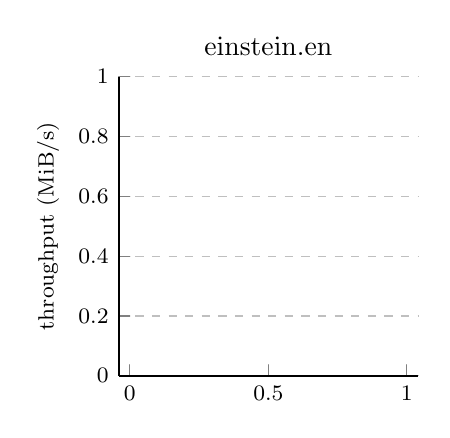
\begin{tikzpicture}
\begin{axis}[
  title={einstein.en},
  ylabel={throughput (MiB/s)},
  %ymode=log,
  plotConstructionWoRs,
]
%% MULTIPLOT(algorithm|attr|ptitle)
%% SELECT (space_usage*8.0)/prefix_size AS x, (prefix_size/1024.0/1024.0)/AVG(construction_time_ms/1000.0) AS y, plot_attr AS attr, plot_name AS ptitle, sorting_order AS sorting_order, MULTIPLOT
%% FROM our_stats
%% JOIN algorithm_meta_data ON algorithm = algorithm_name
%% WHERE input LIKE '%einstein.en.txt%'
%%GROUP BY MULTIPLOT,x ORDER BY sorting_order
\addplot[mark=asterisk,color=fp1Color] coordinates { (0.0131831,0.554619) (0.01479,0.564117) (0.0175022,0.575552) (0.0182833,1.08143) (0.0212268,0.58774) (0.0214105,1.12037) (0.0254528,1.49635) (0.0323534,1.15955) (0.0361695,2.10782) (0.0376881,1.58698) (0.0839268,2.25455) };
\addlegendentry{FP$_1$};
\addplot[mark=triangle,color=lpfzColor] coordinates { (0.0152427,4.61362) (0.0168498,4.62146) (0.0186902,4.57514) (0.0195619,4.62922) (0.0218173,4.62307) (0.0232864,4.63342) (0.0254481,4.60504) (0.0327603,4.61961) (0.0361695,4.59009) (0.0376834,4.61822) (0.0839268,4.61714) };
\addlegendentry{LPF$_z$};
\addplot[mark=pentagon,color=lpfzdpColor] coordinates { (0.0152427,4.53597) (0.0168498,4.57047) (0.0186902,4.55904) (0.0195619,4.55088) (0.0218173,4.56729) (0.0232864,4.58055) (0.0254481,4.55568) (0.0327603,4.56972) (0.0361695,4.55365) (0.0376834,4.55305) (0.0839268,4.5612) };g
\addlegendentry{LPF$^{\textnormal{DP}}_z$};
\addplot[mark=x,color=lpf1dpColor] coordinates { (0.0131831,4.14882) (0.01479,4.14468) (0.0175022,4.14987) (0.0182833,4.33528) (0.0212268,4.15619) (0.0214105,4.34065) (0.0254528,4.40953) (0.0323534,4.3449) (0.0361695,4.43109) (0.0376881,4.41586) (0.0839268,4.43799) };
\addlegendentry{LPF$^{\textnormal{DP}}_1$};
\addplot[mark=+,color=lpf1Color] coordinates { (0.0131831,4.59758) (0.01479,4.6145) (0.0175022,4.61816) (0.0182833,4.60904) (0.0212268,4.62073) (0.0214105,4.62089) (0.0254528,4.60152) (0.0323534,4.63141) (0.0361695,4.59302) (0.0376881,4.61732) (0.0839268,4.61714) };
\addlegendentry{LPF$_1$};

%% MULTIPLOT(algorithm|attr|ptitle)
%% SELECT (space_usage*8.0)/prefix_size AS x, (prefix_size/1024.0/1024.0)/AVG(construction_time_ms/1000.0) AS y, plot_attr AS attr, plot_name AS ptitle, sorting_order AS sorting_order, MULTIPLOT
%% FROM belazzougui_stats
%% JOIN algorithm_meta_data ON algorithm = algorithm_name
%% WHERE input LIKE '%einstein.en.txt%'
%%GROUP BY MULTIPLOT,x ORDER BY MULTIPLOT,x
\addplot[mark=star,color=belazzouguiColor,scale=.9] coordinates { (0.0149838,0.709471) (0.0176547,0.710077) (0.0213513,0.710466) (0.0215753,1.3255) (0.02535,1.30029) (0.0306332,1.85577) (0.0324724,1.32761) (0.037839,1.78624) (0.0448578,2.27089) (0.0517207,1.84617) (0.0584732,2.16841) (0.08408,2.27973) };
\addlegendentry{original~BT~\cite{belazzougui21block}};

\legend{};

\end{axis}
\end{tikzpicture}
  &
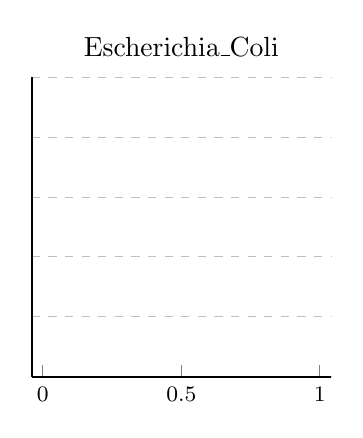
\begin{tikzpicture}
\begin{axis}[
  title={Escherichia\_Coli},
  ymajorticks=false,
  %ymode=log,
  plotConstructionWoRs,
]
%% MULTIPLOT(algorithm|attr|ptitle)
%% SELECT (space_usage*8.0)/prefix_size AS x, (prefix_size/1024.0/1024.0)/AVG(construction_time_ms/1000.0) AS y, plot_attr AS attr, plot_name AS ptitle, sorting_order AS sorting_order, MULTIPLOT
%% FROM our_stats
%% JOIN algorithm_meta_data ON algorithm = algorithm_name
%% WHERE input LIKE '%Escherichia_Coli%'
%%GROUP BY MULTIPLOT,x ORDER BY sorting_order
\addplot[mark=asterisk,color=fp1Color] coordinates { (0.87409,0.375703) (0.876721,0.369596) (1.0141,0.399402) (1.11474,0.433181) (1.11732,0.745905) (1.20232,1.00496) (1.38717,0.883029) (1.39946,1.28071) (1.44333,1.24378) (1.60587,0.720581) (2.12041,1.83481) };
\addlegendentry{FP$_1$};
\addplot[mark=triangle,color=lpfzColor] coordinates { (1.10323,4.48124) (1.10586,3.87383) (1.24334,5.00423) (1.34081,5.03199) (1.35032,5.11571) (1.41265,4.3348) (1.43233,4.94237) (1.66811,5.14307) (1.83248,4.1572) (2.17303,5.12571) };
\addlegendentry{LPF$_z$};
\addplot[mark=pentagon,color=lpfzdpColor] coordinates { (1.10323,4.41672) (1.10586,4.19032) (1.24334,4.6101) (1.34081,4.73015) (1.35032,4.80746) (1.41265,4.60529) (1.43233,4.66295) (1.66811,4.95737) (1.83248,4.41854) (2.17303,4.93785) };
\addlegendentry{LPF$^{\textnormal{DP}}_z$};
\addplot[mark=x,color=lpf1dpColor] coordinates { (0.87409,3.23874) (0.876721,3.1076) (1.0141,3.34548) (1.11474,3.417) (1.11732,3.91195) (1.20232,4.02954) (1.38717,4.07827) (1.39946,4.22032) (1.44333,4.31802) (1.60587,3.71146) (2.12041,4.469) };
\addlegendentry{LPF$^{\textnormal{DP}}_1$};
\addplot[mark=+,color=lpf1Color] coordinates { (0.87409,4.44338) (0.876721,3.82911) (1.0141,4.95424) (1.11474,5.06436) (1.11732,5.01314) (1.20232,4.29725) (1.38717,5.1553) (1.39946,4.92767) (1.44333,5.13948) (1.60587,4.1382) (2.12041,5.11668) };
\addlegendentry{LPF$_1$};

%% MULTIPLOT(algorithm|attr|ptitle)
%% SELECT (space_usage*8.0)/prefix_size AS x, (prefix_size/1024.0/1024.0)/AVG(construction_time_ms/1000.0) AS y, plot_attr AS attr, plot_name AS ptitle, sorting_order AS sorting_order, MULTIPLOT
%% FROM belazzougui_stats
%% JOIN algorithm_meta_data ON algorithm = algorithm_name
%% WHERE input LIKE '%Escherichia_Coli%'
%%GROUP BY MULTIPLOT,x ORDER BY MULTIPLOT,x
\addplot[mark=star,color=belazzouguiColor,scale=.9] coordinates { (0.889746,0.395945) (1.02393,0.412882) (1.12088,0.443414) (1.12512,0.724651) (1.19561,0.784931) (1.27663,1.06654) (1.39006,0.856064) (1.44615,1.16485) (1.49534,1.40776) (1.73921,1.23025) (1.7713,1.53801) (2.12128,1.62289) };
\addlegendentry{original~BT~\cite{belazzougui21block}};

\legend{};

\end{axis}
\end{tikzpicture}
  &
\begin{tikzpicture}
\begin{axis}[
  title={influenza},
  %ymode=log,
  ymajorticks=false,
  plotConstructionWoRs,
]
%% MULTIPLOT(algorithm|attr|ptitle)
%% SELECT (space_usage*8.0)/prefix_size AS x, (prefix_size/1024.0/1024.0)/AVG(construction_time_ms/1000.0) AS y, plot_attr AS attr, plot_name AS ptitle, sorting_order AS sorting_order, MULTIPLOT
%% FROM our_stats
%% JOIN algorithm_meta_data ON algorithm = algorithm_name
%% WHERE input LIKE '%influenza%'
%%GROUP BY MULTIPLOT,x ORDER BY sorting_order
\addplot[mark=asterisk,color=fp1Color] coordinates { (0.337051,0.397877) (0.339243,0.393317) (0.363739,0.404945) (0.457446,0.416419) (0.485128,0.759249) (0.544267,0.744063) (0.734057,1.08759) (0.766695,0.813504) (0.849092,1.18348) (0.867402,1.40938) (1.77759,1.67716) };
\addlegendentry{FP$_1$};
\addplot[mark=triangle,color=lpfzColor] coordinates { (0.3685,4.79107) (0.370691,4.68594) (0.395189,4.97613) (0.488922,5.12533) (0.510723,5.00858) (0.569874,4.73777) (0.734954,4.66922) (0.788642,5.24639) (0.850011,5.19672) (0.869696,4.84511) (1.78116,5.23072) };
\addlegendentry{LPF$_z$};
\addplot[mark=pentagon,color=lpfzdpColor] coordinates { (0.3685,4.77213) (0.370691,4.73585) (0.395189,4.86282) (0.488922,4.96387) (0.510723,4.9703) (0.569874,4.87487) (0.734954,4.85321) (0.788642,5.11309) (0.850011,5.09626) (0.869696,4.90195) (1.78116,5.1174) };g
\addlegendentry{LPF$^{\textnormal{DP}}_z$};
\addplot[mark=x,color=lpf1dpColor] coordinates { (0.337051,3.89838) (0.339243,3.87292) (0.363739,3.95361) (0.457446,4.01245) (0.485128,4.43765) (0.544267,4.35863) (0.734057,4.46588) (0.766695,4.55126) (0.849092,4.68617) (0.867402,4.61004) (1.77759,4.8062) };
\addlegendentry{LPF$^{\textnormal{DP}}_1$};
\addplot[mark=+,color=lpf1Color] coordinates { (0.337051,4.71679) (0.339243,4.60038) (0.363739,4.88611) (0.457446,5.07576) (0.485128,4.9635) (0.544267,4.6853) (0.734057,4.64255) (0.766695,5.19977) (0.849092,5.17937) (0.867402,4.78509) (1.77759,5.20331) };
\addlegendentry{LPF$_1$};

%% MULTIPLOT(algorithm|attr|ptitle)
%% SELECT (space_usage*8.0)/prefix_size AS x, (prefix_size/1024.0/1024.0)/AVG(construction_time_ms/1000.0) AS y, plot_attr AS attr, plot_name AS ptitle, sorting_order AS sorting_order, MULTIPLOT
%% FROM belazzougui_stats
%% JOIN algorithm_meta_data ON algorithm = algorithm_name
%% WHERE input LIKE '%influenza%'
%%GROUP BY MULTIPLOT,x ORDER BY MULTIPLOT,x
\addplot[mark=star,color=belazzouguiColor,scale=.9] coordinates { (0.343194,0.409209) (0.369065,0.413363) (0.461716,0.421918) (0.490159,0.748481) (0.560272,0.771486) (0.671162,1.06204) (0.769398,0.793568) (0.851982,1.08673) (0.932888,1.36514) (1.21869,1.18568) (1.26419,1.46111) (1.77863,1.4901) };
\addlegendentry{original~BT~\cite{belazzougui21block}};

\legend{};

\end{axis}
\end{tikzpicture}
  \\
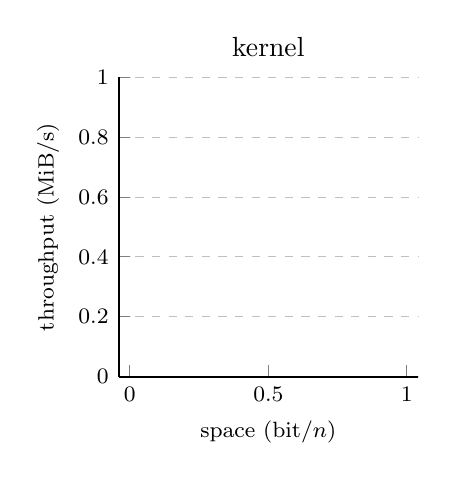
\begin{tikzpicture}
\begin{axis}[
  title={kernel},
  xlabel={space (\(\textnormal{bit}/n\))},
  ylabel={throughput (MiB/s)},
  %ymode=log,
  plotConstructionWoRs,
]
%% MULTIPLOT(algorithm|attr|ptitle)
%% SELECT (space_usage*8.0)/prefix_size AS x, (prefix_size/1024.0/1024.0)/AVG(construction_time_ms/1000.0) AS y, plot_attr AS attr, plot_name AS ptitle, sorting_order AS sorting_order, MULTIPLOT
%% FROM our_stats
%% JOIN algorithm_meta_data ON algorithm = algorithm_name
%% WHERE input LIKE '%kernel%'
%%GROUP BY MULTIPLOT,x ORDER BY sorting_order
\addplot[mark=asterisk,color=fp1Color] coordinates { (0.161156,0.582592) (0.183612,0.598104) (0.214568,1.10834) (0.237924,1.61436) (0.246371,0.622138) (0.26208,1.1678) (0.300593,0.644741) (0.31586,2.10227) (0.359495,1.25563) (0.377103,1.8192) (0.550211,2.47096) };
\addlegendentry{FP$_1$};
\addplot[mark=triangle,color=lpfzColor] coordinates { (0.210718,5.25875) (0.233173,5.3916) (0.238155,5.31457) (0.285693,5.45176) (0.287756,5.40516) (0.295935,5.45302) (0.320572,5.43169) (0.350166,5.47219) (0.383856,5.48093) (0.429652,5.46969) (0.55743,5.46866) };
\addlegendentry{LPF$_z$};
\addplot[mark=pentagon,color=lpfzdpColor] coordinates { (0.210718,5.20898) (0.233173,5.27442) (0.238155,5.26667) (0.285693,5.32371) (0.287756,5.29708) (0.295935,5.30144) (0.320572,5.32292) (0.350166,5.34641) (0.383856,5.38503) (0.429652,5.35755) (0.55743,5.37816) };g
\addlegendentry{LPF$^{\textnormal{DP}}_z$};
\addplot[mark=x,color=lpf1dpColor] coordinates { (0.161156,4.62607) (0.183612,4.65114) (0.214568,4.92295) (0.237924,5.03635) (0.246371,4.72678) (0.26208,4.99549) (0.300593,4.73211) (0.31586,5.14111) (0.359495,5.04359) (0.377103,5.10471) (0.550211,5.19534) };
\addlegendentry{LPF$^{\textnormal{DP}}_1$};
\addplot[mark=+,color=lpf1Color] coordinates { (0.161156,5.23841) (0.183612,5.38735) (0.214568,5.2864) (0.237924,5.37182) (0.246371,5.44956) (0.26208,5.46287) (0.300593,5.45492) (0.31586,5.42934) (0.359495,5.47678) (0.377103,5.4837) (0.550211,5.47028) };
\addlegendentry{LPF$_1$};

%% MULTIPLOT(algorithm|attr|ptitle)
%% SELECT (space_usage*8.0)/prefix_size AS x, (prefix_size/1024.0/1024.0)/AVG(construction_time_ms/1000.0) AS y, plot_attr AS attr, plot_name AS ptitle, sorting_order AS sorting_order, MULTIPLOT
%% FROM belazzougui_stats
%% JOIN algorithm_meta_data ON algorithm = algorithm_name
%% WHERE input LIKE '%kernel%'
%%GROUP BY MULTIPLOT,x ORDER BY MULTIPLOT,x
\addplot[mark=star,color=belazzouguiColor,scale=.9] coordinates { (0.185815,0.744318) (0.247742,0.755522) (0.263176,1.38605) (0.301419,0.765629) (0.313855,1.3922) (0.331991,1.89217) (0.359933,1.42621) (0.377586,1.96182) (0.398629,2.37201) (0.435837,2.00502) (0.458434,2.49146) (0.550488,2.49576) };
\addlegendentry{original~BT~\cite{belazzougui21block}};

\legend{};

\end{axis}
\end{tikzpicture}
  &
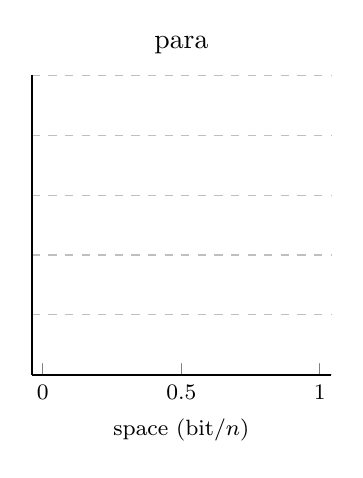
\begin{tikzpicture}
\begin{axis}[
  title={para},
  xlabel={space (\(\textnormal{bit}/n\))},
  %ymode=log,
  ymajorticks=false,
  plotConstructionWoRs,
]
%% MULTIPLOT(algorithm|attr|ptitle)
%% SELECT (space_usage*8.0)/prefix_size AS x, (prefix_size/1024.0/1024.0)/AVG(construction_time_ms/1000.0) AS y, plot_attr AS attr, plot_name AS ptitle, sorting_order AS sorting_order, MULTIPLOT
%% FROM our_stats
%% JOIN algorithm_meta_data ON algorithm = algorithm_name
%% WHERE input LIKE '%para%'
%%GROUP BY MULTIPLOT,x ORDER BY sorting_order
\addplot[mark=asterisk,color=fp1Color] coordinates { (0.281326,0.38514) (0.294562,0.370528) (0.296383,0.367396) (0.305995,0.405652) (0.337317,0.744424) (0.399985,0.821028) (0.444005,1.12314) (0.485358,0.988906) (0.518785,1.35086) (0.531368,0.726367) (0.703199,1.69826) };
\addlegendentry{FP$_1$};
\addplot[mark=triangle,color=lpfzColor] coordinates { (0.351498,4.67243) (0.364733,4.4957) (0.366553,4.29866) (0.376181,4.71886) (0.399255,4.68951) (0.457638,4.73181) (0.462919,4.75007) (0.499082,4.409) (0.54769,4.64748) (0.593526,4.40375) (0.735488,4.73684) };
\addlegendentry{LPF$_z$};
\addplot[mark=pentagon,color=lpfzdpColor] coordinates { (0.351498,4.48547) (0.364733,4.4244) (0.366553,4.35529) (0.376181,4.54834) (0.399255,4.54356) (0.457638,4.61104) (0.462919,4.62449) (0.499082,4.48818) (0.54769,4.5301) (0.593526,4.44955) (0.735488,4.65273) };g
\addlegendentry{LPF$^{\textnormal{DP}}_z$};
\addplot[mark=x,color=lpf1dpColor] coordinates { (0.281326,3.69301) (0.294562,3.65322) (0.296383,3.60615) (0.305995,3.74398) (0.337317,4.0808) (0.399985,4.15139) (0.444005,4.2681) (0.485358,4.1636) (0.518785,4.24263) (0.531368,4.00293) (0.703199,4.34877) };
\addlegendentry{LPF$^{\textnormal{DP}}_1$};
\addplot[mark=+,color=lpf1Color] coordinates { (0.281326,4.60277) (0.294562,4.4508) (0.296383,4.22596) (0.305995,4.68214) (0.337317,4.64934) (0.399985,4.72854) (0.444005,4.6965) (0.485358,4.36144) (0.518785,4.57141) (0.531368,4.33417) (0.703199,4.70854) };
\addlegendentry{LPF$_1$};

%% MULTIPLOT(algorithm|attr|ptitle)
%% SELECT (space_usage*8.0)/prefix_size AS x, (prefix_size/1024.0/1024.0)/AVG(construction_time_ms/1000.0) AS y, plot_attr AS attr, plot_name AS ptitle, sorting_order AS sorting_order, MULTIPLOT
%% FROM belazzougui_stats
%% JOIN algorithm_meta_data ON algorithm = algorithm_name
%% WHERE input LIKE '%para%'
%%GROUP BY MULTIPLOT,x ORDER BY MULTIPLOT,x
\addplot[mark=star,color=belazzouguiColor,scale=.9] coordinates { (0.284957,0.43069) (0.299815,0.424454) (0.308479,0.44169) (0.340391,0.790842) (0.349348,0.787788) (0.40142,0.838103) (0.408417,1.08579) (0.445577,1.11269) (0.503648,1.34647) (0.531659,1.17507) (0.574126,1.35312) (0.704017,1.49929) };
\addlegendentry{original~BT~\cite{belazzougui21block}};

\legend{};

\end{axis}
\end{tikzpicture}
  &
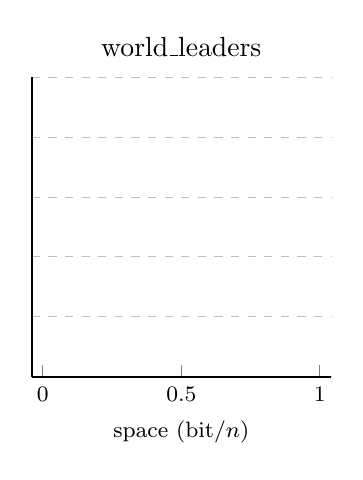
\begin{tikzpicture}
\begin{axis}[
  title={world\_leaders},
  xlabel={space (\(\textnormal{bit}/n\))},
  %ymode=log,
  ymajorticks=false,
  plotConstructionWoRs,
]
%% MULTIPLOT(algorithm|attr|ptitle)
%% SELECT (space_usage*8.0)/prefix_size AS x, (prefix_size/1024.0/1024.0)/AVG(construction_time_ms/1000.0) AS y, plot_attr AS attr, plot_name AS ptitle, sorting_order AS sorting_order, MULTIPLOT
%% FROM our_stats
%% JOIN algorithm_meta_data ON algorithm = algorithm_name
%% WHERE input LIKE '%world_leaders%'
%%GROUP BY MULTIPLOT,x ORDER BY sorting_order
\addplot[mark=asterisk,color=fp1Color] coordinates { (0.23667,0.55553) (0.251215,0.564664) (0.298814,0.57592) (0.33278,1.03546) (0.365519,1.07462) (0.396476,0.586495) (0.438749,1.4558) (0.592318,1.8996) (0.647437,1.12788) (0.714122,1.58169) (1.64432,2.18905) };
\addlegendentry{FP$_1$};
\addplot[mark=triangle,color=lpfzColor] coordinates { (0.257885,5.81517) (0.272434,5.98855) (0.320033,6.06668) (0.338224,5.86083) (0.370969,6.07656) (0.417726,6.1309) (0.452455,5.9363) (0.592456,5.8792) (0.653304,6.11472) (0.729457,6.17088) (1.64463,6.12782) };
\addlegendentry{LPF$_z$};
\addplot[mark=pentagon,color=lpfzdpColor] coordinates { (0.257885,5.76429) (0.272434,5.82955) (0.320033,5.90642) (0.338224,5.82299) (0.370969,5.94391) (0.417726,5.95617) (0.452455,5.91045) (0.592456,5.88032) (0.653304,6.02399) (0.729457,6.04363) (1.64463,5.99764) };g
\addlegendentry{LPF$^{\textnormal{DP}}_z$};
\addplot[mark=x,color=lpf1dpColor] coordinates { (0.23667,4.90803) (0.251215,4.98635) (0.298814,5.06433) (0.33278,5.37487) (0.365519,5.48254) (0.396476,5.10009) (0.438749,5.55484) (0.592318,5.63316) (0.647437,5.56173) (0.714122,5.68239) (1.64432,5.73477) };
\addlegendentry{LPF$^{\textnormal{DP}}_1$};
\addplot[mark=+,color=lpf1Color] coordinates { (0.23667,5.82576) (0.251215,5.92439) (0.298814,5.96039) (0.33278,5.82374) (0.365519,6.05984) (0.396476,6.08344) (0.438749,5.87942) (0.592318,5.85393) (0.647437,6.15561) (0.714122,6.11917) (1.64432,6.13622) };
\addlegendentry{LPF$_1$};

%% MULTIPLOT(algorithm|attr|ptitle)
%% SELECT (space_usage*8.0)/prefix_size AS x, (prefix_size/1024.0/1024.0)/AVG(construction_time_ms/1000.0) AS y, plot_attr AS attr, plot_name AS ptitle, sorting_order AS sorting_order, MULTIPLOT
%% FROM belazzougui_stats
%% JOIN algorithm_meta_data ON algorithm = algorithm_name
%% WHERE input LIKE '%world_leaders%'
%%GROUP BY MULTIPLOT,x ORDER BY MULTIPLOT,x
\addplot[mark=star,color=belazzouguiColor,scale=.9] coordinates { (0.254912,0.614697) (0.301726,0.621437) (0.36836,1.11918) (0.398709,0.628559) (0.46728,1.14826) (0.549244,1.55197) (0.649067,1.15695) (0.715983,1.58146) (0.789572,1.93046) (1.07136,1.63337) (1.12837,1.94724) (1.64534,2.02855) };
\addlegendentry{original~BT~\cite{belazzougui21block}};

\legend{};

\end{axis}
\end{tikzpicture}
\end{tabular}

\end{document}
